%%%%%%%%%%%%%%%%%%%%%%%%%%%%%%%%%%%%%%%%%%%%%%%%%%%%%%%%%%
% Acoustics and Music Technology Final Project Latex Template
%
% CHAPTER 3 PAGE
%
% TOTAL EDITS REQUIRED: 1
%
% NOTE: NO NEED TO INCLUDE ANY FURTHER PREAMBLE IN THIS FILE
%%%%%%%%%%%%%%%%%%%%%%%%%%%%%%%%%%%%%%%%%%%%%%%%%%%%%%%%%%

\chapter{Analysis: Magpie}\label{analysis-magpie}

\section{The Problem}\label{the-problem-2}

\subsection{Plate Theory}\label{plate-theory}

\subsection{Boundary Conditions}\label{boundary-conditions}

\section{The Solution}\label{the-solution-1}

\subsection{Implementation}\label{implementation}

\subsubsection{Discretising}\label{discretising}
\subsubsection{Design}\label{design}

\section{Application}\label{application-1}
%%%%%%%%%%%% EDIT %%%%%%%%%%%%

\chapter{2D wave equation}
\label{chapter3}
\section{2D wave equation}
\label{chapter3:sec1}
The discussion of this chapter will be mainly focused on the wave equation. This simple second order partial differential equation describes the motion of waves over a domain \textit{D}. It is defined as follows,
\begin{equation}
\label{eqn:wave}
	u_{tt}=c^{2}\nabla u
\end{equation} 
Where $u_{tt}$ represents the second order partial derivative with respect to time $t$, $c$ is the wave speed and $\nabla u$ represent the Laplacian operator over $u$. Before the study on the wave equation continuous it is necessary to define the Laplacian operator.\\
The Laplacian operator $\nabla$ can operate on $u$ on different dimensions dependent of the variables affecting $u$. If we consider for example $u$ to be a 3D vector, we can describe the Lapalacian operation on $u$ by the following equation
\begin{equation}
	\nabla u = \frac{\partial^2}{\partial xx}u + \frac{\partial^{2}}{\partial yy}u + \frac{\partial^{2}}{\partial zz}
\end{equation}
Thus, if we want to operate in lower dimensions say 1D or 2D, it will only be necessary to define the operator over 1 or 2 variables resprectively.\\
It is possible now to rearrange Eq.\ref{eqn:wave} for a two dimensional domain \textit{D} to achieve the equation,
\begin{equation}
	u_{tt}=c^{2}( \frac{\partial^2}{\partial xx}u + \frac{\partial^{2}}{\partial yy}u)	
\end{equation}
 If we consider \textit{D} to be of finite dimension, we can rearrange the above expression as
\begin{equation}
\label{eqn:wave2}
	\begin{aligned}
	u_{tt}=\gamma^{2}(\frac{\partial^2}{\partial xx}u + \frac{\partial^{2}}{\partial yy}u)
	\end{aligned}
\end{equation}
Where $\gamma=c/L$ and $L=\sqrt{|D|}$.\\
\subsection{Exact solution and analysis}
\label{chapter3:sec1:ssec1}
This particular kind of PDE admits an exact solution of the form $u(x,y,t)=\e^{st+j(\beta_{x}x+\beta_{y}y)}$, therefore, if we introduce this solution into \ref{eqn:wave2}, this yields,
\begin{equation}
		s^{2}=-\gamma^{2}(\beta_{x}^{2}+\beta_{y}^{2})
\end{equation}
From which we can reach the dispersion relation,
\begin{equation}
	\begin{aligned}
	\omega=\pm \gamma|\mathrm{\beta}| \ \ \ \ \     \text{where} \ \ \ \ \     |\mathrm{\beta}|=\sqrt{(\beta_{x}^{2}+\beta_{y}^{2})}
	\end{aligned}
\end{equation}
And so we can derive the expressions for phase and group velocity $\textit{v}_{\phi}$ and $\textit{v}_{g}$
\begin{equation}
	\begin{aligned*}
		\textit{v}_{\phi}&=\frac{\omega}{\mathrm{\beta}}&=\gamma \ \  
		\textit{v}_{g}&=\frac{\partial \omega}{\partial\mathrm{\beta}}&=\gamma
	\end{aligned*}
\end{equation}
We can see by the above equations that all the waves will travel at the same speed independently of frequency and wavenumber. This kind of behaviour is defined as $\textit{nondispersive}$.
\subsection{Initial and boundary conditions}
\label{chapter3:sec1:ssec2}
In order to initialise this PDE, it is necessary to define a set of initial conditions. These are normally defined by an initial displacement $u(x,y,0)=u_{0}(x,y)$ and an initial velocity $(\partia u/ \partial t)=v_{0}(x,y)$ but for purposes of this paper this set of initial conditions are not required given that the wave equation will be driven by force $f(t)$.\\ 
Considering the fact that this wave propagation is produced over a finite domain, it is necessary to introduce a set of conditions to determine the different behaviour at the boundaries.\\
Two typical conditions are defined by the following equations
\begin{equation}
	u(0,y,t)=0 \\\\\ u_{x}(0,y,t)=0
\end{equation}
Which are refered as Dirichlet and Neumann conditions respectively. The former will represent the behaviour of the boundaries when this are fixed while the later will represent a fixed behaviour. For purposes of this paper, we will consider that the boundaries of our domain behave under Dirichlet conditions, this is due to the simplicity of imposing such condition.
\section{2D wave equation using FDTD}
\label{chapter3:sec1}
The study will continue by approximating the above equations using FDTD schemes. There are different ways of approximating this equation depending on the approximation to the Laplace operator. This paper will cover two ways of approximating $\nabla$ in cartesian coordinates, a five point approximation and a nine point approximation.
\subsection{Five point approximation}
\label{chapter3:sec1:ssec1}
One way to approximate the 2D Laplacian operator is to use a five point stencil. By a five point stencil, we refer to the fact that to produce an approximation to $\nabla$ at a particular point $u_{(x,y)}^{n}$, we will take in consideration two neighbouring points of $u_{(x,y)}^{n}$ with respect to each coordinate.\\
If we consider that $\frac{\partial^{2}}{\partial xx}\cong\delta_{xx}$ as define in Eq.\ref{eqn:ddiff} we can defined $\delta_{\delta\boxplus}$ as
\begin{equation}
	\delta_{\delta\boxplus}=\delta_{xx}+\delta{yy}\cong \Delta
\end{equation}
Equation \ref{eqn:wave2} can therefore be expressed as follows
\begin{equation}
	\delta_{tt}u=\gamma^{2}\delta_{\Delta\boxplus}u
\end{equation}
\begin{figure}[tb!]
\begin{center}
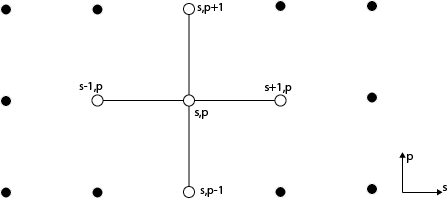
\includegraphics[width=10cm]{./Chapter_3/_Figs/5point.png}
\caption{Five point stencil for a given point at location (s,p) in a two dimensional grid.}
\label{figs:5point}
\end{center}
\end{figure}
Where $u=u^{n}_{x,y}$  which represent a two dimensional grid where each point is represented by a particula choice of integers $x$ and $y$. $x$ and $y$ in this case will represent the approximation to the points $x=xh_{x}$ and $y=yh_{y}$ where $h_{x}$ and $h_{y}$ represent the grid spacing on the $X$ and $Y$ coordinates resprectively. For simplicity in this paper, we will consider an equally spaced grid, thus $h=h_{x}=h_{y}$.\\
Expanding the above expression we yield the following equation
\begin{equation}
	\frac{1}{k^2}(u^{n+1}_{x,y}-2u^{n}_{x,y}+u^{n-1}_{x,y}=\gamma^{2}\frac{1}{h^2}((u^{n}_{x+1,y}-2u^{n}_{x,y}+u^{n}_{x-1,y})+(u^{n}_{x,y+1}-2u^{n}_{x,y}+u^{n}_{x,y-1}))\\
\end{equation}
Which can be rearranged to
\begin{equation}
\label{eqn:FD5wave}
	u^{n+1}_{x,y}=2u^{n}_{x,y}-u^{n-1}_{x,y}+\lambda^{2}(u^{n}_{x+1,y}+u^{n}_{x-1,y}+u^{n}_{x,y+1}+u^{n}_{x,y-1}-4u^{n}_{x,y})
\end{equation}
For $\lambda=\frac{k\gamma}{h}$.\\
It is worth noting that there is a condition that must be impossed to $\lambda$ so that the solution is stable. This condition is developed by using Von Neumann analysis on \ref{eqn:FD5wave} using the solution $u^{n}_{s,p}=z^{n}\e^{jh(s\beta_{x}+p\beta_{y}})$ and solving for $z$. Since $z$ must satisfy to be unit modulus,$\lambda$ must satisfy $\lambda\leq \frac{1}{\sqrt{2}}$ (for further explanation see Bilbao).
\subsection{Nine point approximation}
\label{chapter3:sec1:ssec2}

In order to get a more accurate approximation, we can use stencils with a higher number of points, say a nine point interpolation. This kind of method will require a higher computational cost but it will increase the level of nondispersivity of the model with respect to the five point stencil approximation.
In order to develope the nine point approximation we will need to define first another type of operator represented by $\delta_{\Delta\boxtimes}$ which is defined by
\begin{equation}
	\delta_{\Delta\boxtimes}=\delta_{xx}+\delta_{yy} +\frac{h^2}{2}\delta_{xx}\delta_{yy}
\end{equation}
This leads to
\begin{equation}
	\delta_{tt}u=\gamma^{2}(\alpha\delta_{\Delta\boxplus} u + (1-\alpha)\delta_{\Delta\boxtimes}u)
\end {equation}
Which can be rearranged using similar techiniques of Eq.\ref{eqn:FD5wave} to
\begin{figure}[tb!]
\begin{center}
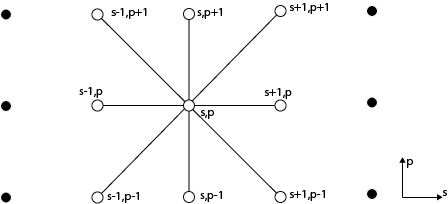
\includegraphics[width=10cm]{./Chapter_3/_Figs/9point.png}
\caption{Nine point stencil for a given point at location (s,p) in a two dimensional grid.}
\label{figs:9point}
\end{center}
\end{figure}
\begin{equation}
\label{eqn:FD9wave}
	\begin{align}
		u^{n+1}_{s,p}&=2u^{n}_{x,y}-u^{n-1}_{x,y}+\lamba^{2}(u^{n}_{x+1,y}+u^{n}_{x-1,y}+u^{n}_{x,y+1}+u^{n}_{x,y-1}-4u^{n}_{x,y}\\
				    &+(\frac{1}{2}(1-\alpha))(u^{n}_{x+1,y+1}+u^{n}_{x+1,y-1}+u^{n}_{x-1,y+1}+u^{n}_{x-1,y-1}\\
				    & -2(u^{n}_{x+1,y}+u^{n}_{x-1,y}+u^{n}_{x,y+1}+u^{n}_{x,y-1})+4u^{n}_{x,y} )
	\end{align}
\end{equation}
Once again if we apply von Neumann analysis to the above expression, we will yield a stability condition on $\lambda$ which is,
\begin{equation}
	\alpha \geq 0  \ \ \ \ \text{and} \ \ \ \ \    \lambda\leq min(1,\frac{1}{\sqrt{2\alpha}}) 
\end{equation}
After some analysis on the accuracy of nine point approximation, results show a better nondispersive behaivour when $\alpha$ sits between the values of 0.6 and 0.8.(Bilbao).\\
It is also worth noting the fact that for $\alpha=1$ this kind of approximation will result in a five point approximation. It can be therefore considered as the general formula for both kinds of approximations.\\

%%%%%%%%%%%% EDIT %%%%%%%%%%%%